\documentclass[hidelinks, 12pt,a4paper]{article}
\usepackage[utf8]{inputenc}
\usepackage[T1]{fontenc}
\usepackage[a4paper,left=2cm,right=2cm,top=2cm,bottom=2cm]{geometry}
\usepackage[english,francais]{babel}
\usepackage[french]{varioref}
\usepackage{libertine}
\usepackage[pdftex]{graphicx}
\usepackage{geometry}
\usepackage[pdftex]{graphicx}
\usepackage{adjustbox}
\usepackage{color}
\usepackage{setspace}
\usepackage{hyperref}
\usepackage{comment}
\usepackage{fancyhdr}
\pagestyle{fancy}

\setlength{\parindent}{0cm}
\setlength{\parskip}{1ex plus 0.5ex minus 0.2ex}
\newcommand{\hsp}{\hspace{20pt}}
\newcommand{\HRule}{\rule{\linewidth}{0.5mm}}

\renewcommand{\baselinestretch}{1.3}
\renewcommand{\headrulewidth}{1pt}
\fancyhead[L]{}
\fancyhead[C]{\textbf{Le Petit Scientifique}}
\fancyhead[R]{
\includegraphics[width=2.5cm]{images/universite-rouen.jpg}}

\begin{document}

\begin{titlepage}
  \begin{sffamily}
  \begin{center}

    % Upper part of the page. The '~' is needed because \\
    % only works if a paragraph has started.

    \textsc{\LARGE UFR des Sciences et Techniques}\\[2.5cm]

    \textsc{\Large Rapport Mini projet LW1 – sCiMS}\\[1.5cm]

    % Title
    \HRule \\[0.4cm]
    { \huge \bfseries Le Petit Scientifique\\[0.4cm] }

	\HRule \\[2cm]
    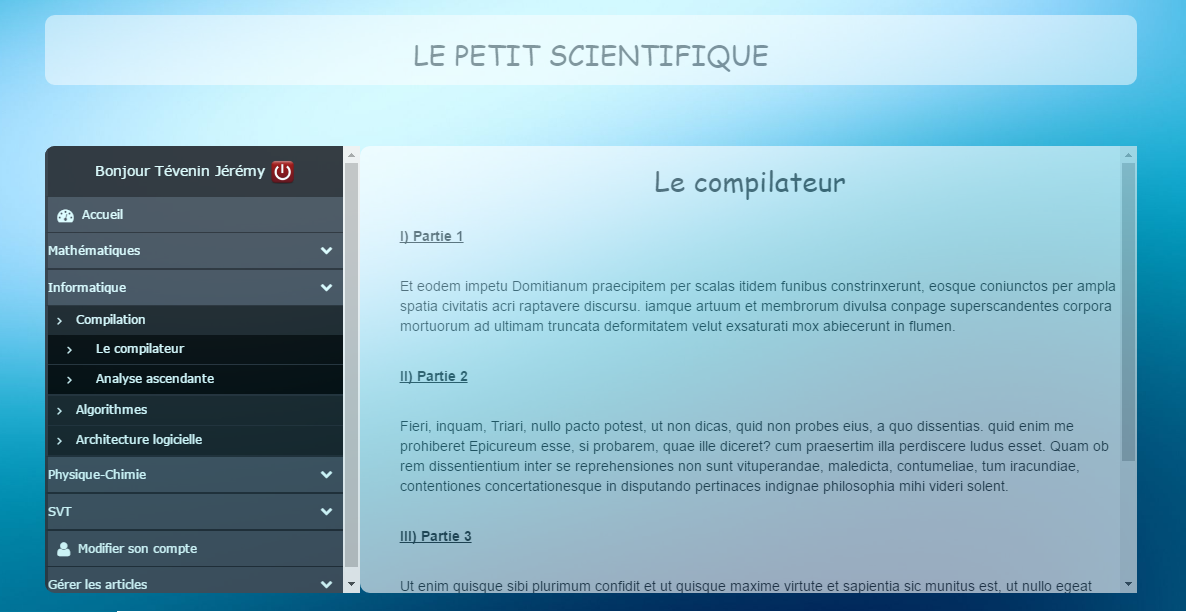
\includegraphics[scale=0.5]{images/accueil2.png}
    \\[2cm]

    % Author and supervisor
    \begin{minipage}{0.4\textwidth}
      \begin{flushleft} \large
        Amine \textsc{BOUAZIZ}\\
        Jérémy \textsc{TEVENIN}\\
      \end{flushleft}
    \end{minipage}
    \begin{minipage}{0.4\textwidth}
      \begin{flushright} \large
        \emph{Rendu à :} M. \textsc{Mallet}\\
      \end{flushright}
    \end{minipage}

    \vfill

    % Bottom of the page
    {\large 22 décembre 2016}

  \end{center}
  \end{sffamily}
\end{titlepage}

\newpage
%Table of contents
\tableofcontents

\newpage
\section{Introduction}
Le projet consiste en l'écriture d'un mini CMS pour la mise en ligne d'articles à caractère scientifique.

Le site sera divisé en catégories, sous-catégories et articles pour organiser le contenu.
Il y a 3 types d'utilisateurs ~:\\ 
\begin{itemize}
\item l'administrateur peut gérer les catégories, sous-catégories et rédacteurs
\item les rédacteurs peuvent ajouter des articles et ils peuvent aussi modifier ou supprimer leur propre articles 
\item les simples utilisateurs peuvent juste visionner les articles
\end{itemize}

\newpage
\section{Manuel d'utilisation}
Pour lancer le site, nous utilisons un serveur wamp. Il suffit de placer le dossier de notre projet dans le dossier de votre serveur.\\

Nous vous fournissons des fichiers sql contenant nos deux bases de données (AUTEUR et MENU). Elles se trouvent dans le dossier ``Bases\_de\_données''.\\

Il vous suffit d'importer ces fichiers sql et de lancer index.php qui vous redirigera vers la page d'accueil.\\

Les identifiants de connexion à la base sont par défaut ``root'' et le mot de passe est vide. Si votre serveur à des identifiants différents, vous trouverez un fichier config.php où vous changerez les identifiants ``USER'' ET ``PASSWD''.\\

\begin{tabbing}
\hspace{2cm}\=\hspace{2cm}\=\kill
<?php\\
\>	define('HOSTNAME','localhost');\\
\>	define('USER','root');\\
\>	define('PASSWD','');\\
\>	define('DBMENU','menu');\\
\>	define('DBAUTEUR','auteur');\\
?>\\
\end{tabbing} 
Vous pourrez vous connecter en mode administrateur en vous connectant avec ~:
\begin{itemize}
\item admin@admin.fr
\item Admin0\\
\end{itemize}

Ou en se connectant avec un rédacteur avec ~:
\begin{itemize}
\item jeremy\_tevenin@hotmail.fr
\item Jeremy76\\
\end{itemize}

(Attention aux majuscules !)\\

Vous pouvez aussi créer votre propre rédacteur ou simplement lire les articles sur le site.

\newpage
\section{Conception}
Pour concevoir notre application, nous avons utilisé un modèle MVC. Notre application contient deux parties différentes ~:
\begin{itemize}
\item la partie accueil permettant de se connecter ou de s'inscrire
\item la partie site permettant de lire les articles ou de les administrer\\
\end{itemize}

Comme nous avons deux parties, nous avons deux contrôleurs différents, acceuil.php et lepetitscientifique.php.\\

Voici un schéma de notre application.\\

\begin{center}
\includegraphics[width=16cm]{images/diag.png}\\
\end{center}

Nous avons aussi un dossier images contenant les images du site, un dossier articles qui contient les articles du site.\\

\newpage
\begin{center}
\textsc{Maquette du site}\\
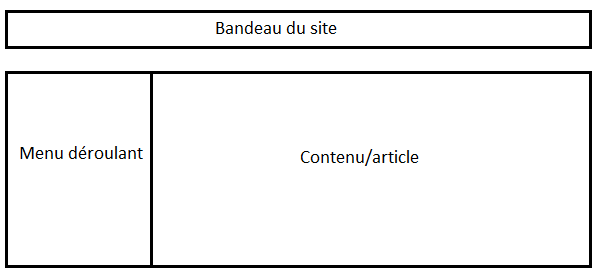
\includegraphics[width=16cm]{images/maquette.png}\\
\end{center}
 
\newpage
\section{Les bases de données}
\subsection{Menu}
La base de données MENU contient toutes les catégories, sous-catégories et articles.\\

Table categorie ~:
\begin{itemize}
\item id auto-incrémenté
\item nom\\
\end{itemize}

Table souscategorie ~:
\begin{itemize}
\item id de référence à categorie
\item id auto-incrémenté
\item nom\\
\end{itemize}

Table article ~: 
\begin{itemize}
\item id de référence à souscategorie
\item id auteur
\item id auto-incrémenté
\item date
\item nom
\item repertoire permet de savoir où est stocké l'article
\item url permet de savoir le nom de l'article\\
\end{itemize}

\subsection{Auteur}

Table auteur ~:
\begin{itemize}
\item id auto-incrémenté
\item nom
\item ville
\item mail qui va permettre la connexion au site
\item un mot de passe
\item un booléen qui détermine le niveau d'administration\\
\end{itemize}

\newpage
\section{Inscription/connexion}
Un utilisateur peut se connecter s'il a déjà un compte, s'inscrire pour devenir rédacteur ou simplement visiter le site.

\subsection{Inscription}
Pour s'inscrire sur le site, il doit remplir un formulaire. Tout se passe sur la page d'accueil où l'utilisateur peut remplir ce formulaire ~:\\

\begin{center}
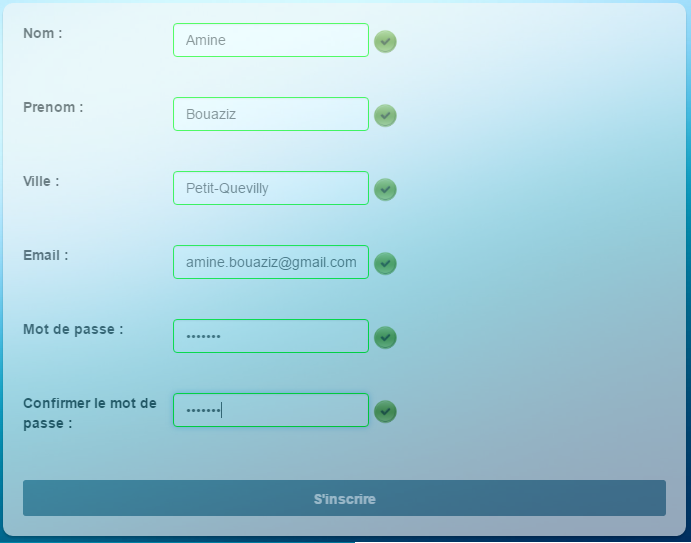
\includegraphics[scale=0.8]{images/inscriptionvalid.png} 
\end{center}

Il doit remplir tous les champs pour pouvoir envoyer le formulaire ! Tant qu'il n'a pas rempli tous les champs, le formulaire ne peut pas être envoyé. Pour cela, nous avons utilisé les fonctionnalités de JQuery. Chaque input est géré par des fonctions gérant la couleur et les messages d'erreurs. C’est le fichier script.js qui gère tout cela. Il y a aussi des sécurités avec des patterns, required et des htmlspecialchar sur les variables reçues.
Le mot de passe est hashé avec la méthode password\_hash() avant d'être mis dans la base de données.\\


\begin{center}
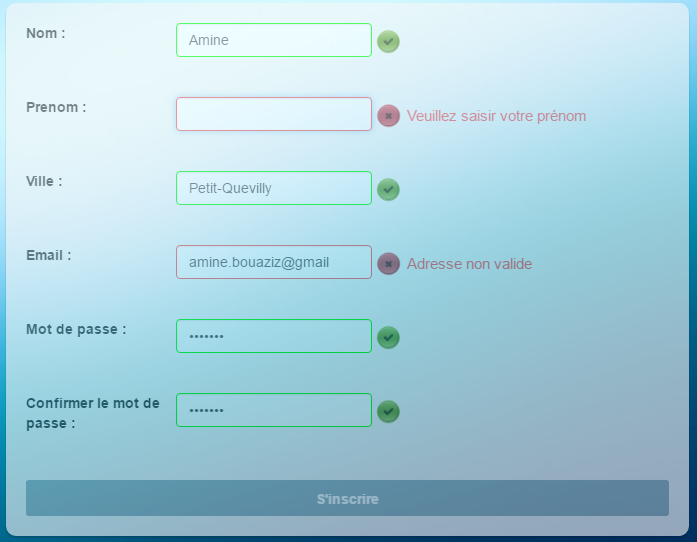
\includegraphics[scale=0.8]{images/inscriptionnnvalid.png}\\
\end{center}

Lors de l'inscription, l'utilisateur est alerté si jamais il utilise une adresse mail déjà existante. Une fois inscrit, il est automatiquement redirigé vers la page lepetitscientifique.php.

\newpage
\subsection{Connexion}
Un utilisateur peut se connecter en remplissant le formulaire suivant ~:\\

\begin{center}
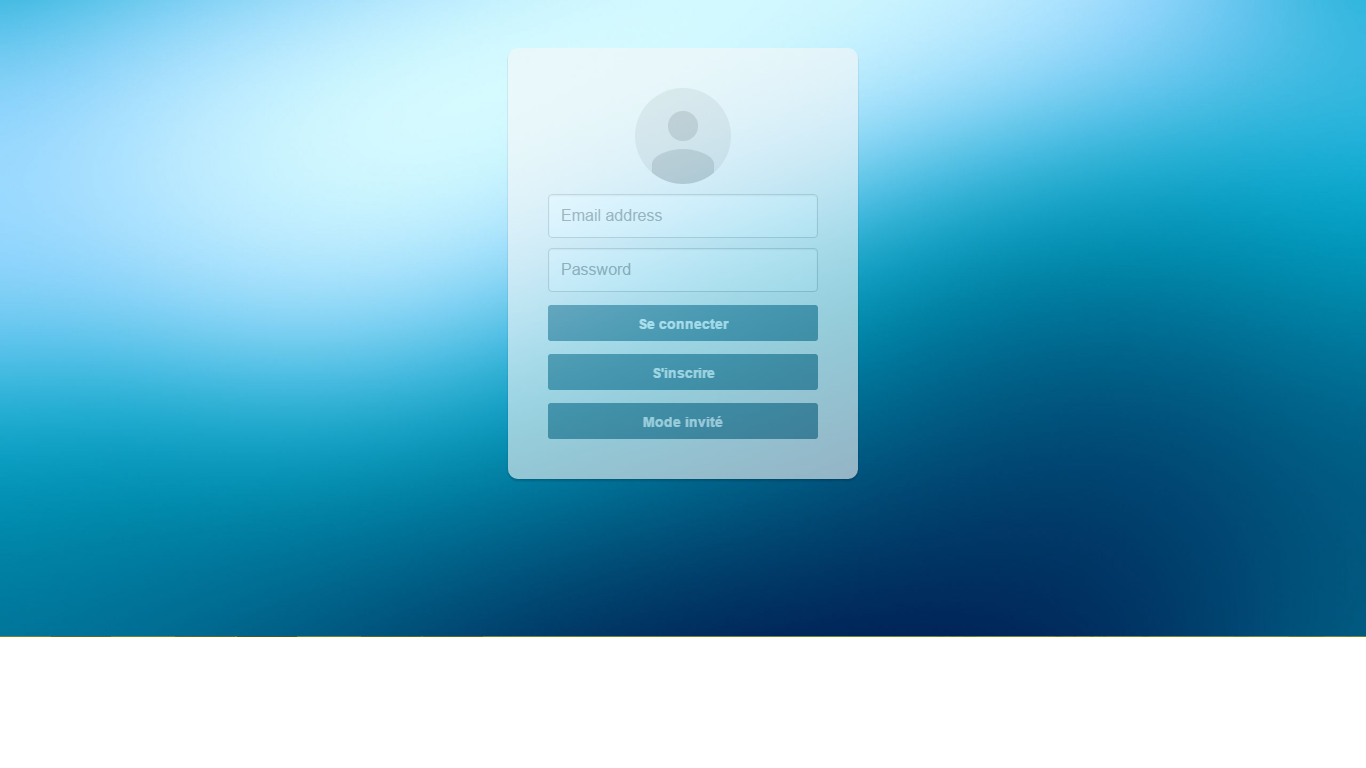
\includegraphics[scale=0.8]{images/connexion.png}\\
\end{center}

Il y a les mêmes sécurités au niveau de la connexion.\\
Lorsqu'il se connecte, en fonction de ses droits, l'utilisateur peut administrer le site.

\newpage
\section{Administration du site}
\subsection{Par l'administrateur}
L'administrateur peut gérer toutes les catégories, sous-catégories et les rédacteurs. 

\subsubsection{Gérer le menu}
\begin{center}
\textsc{Menu de l'administrateur}\\
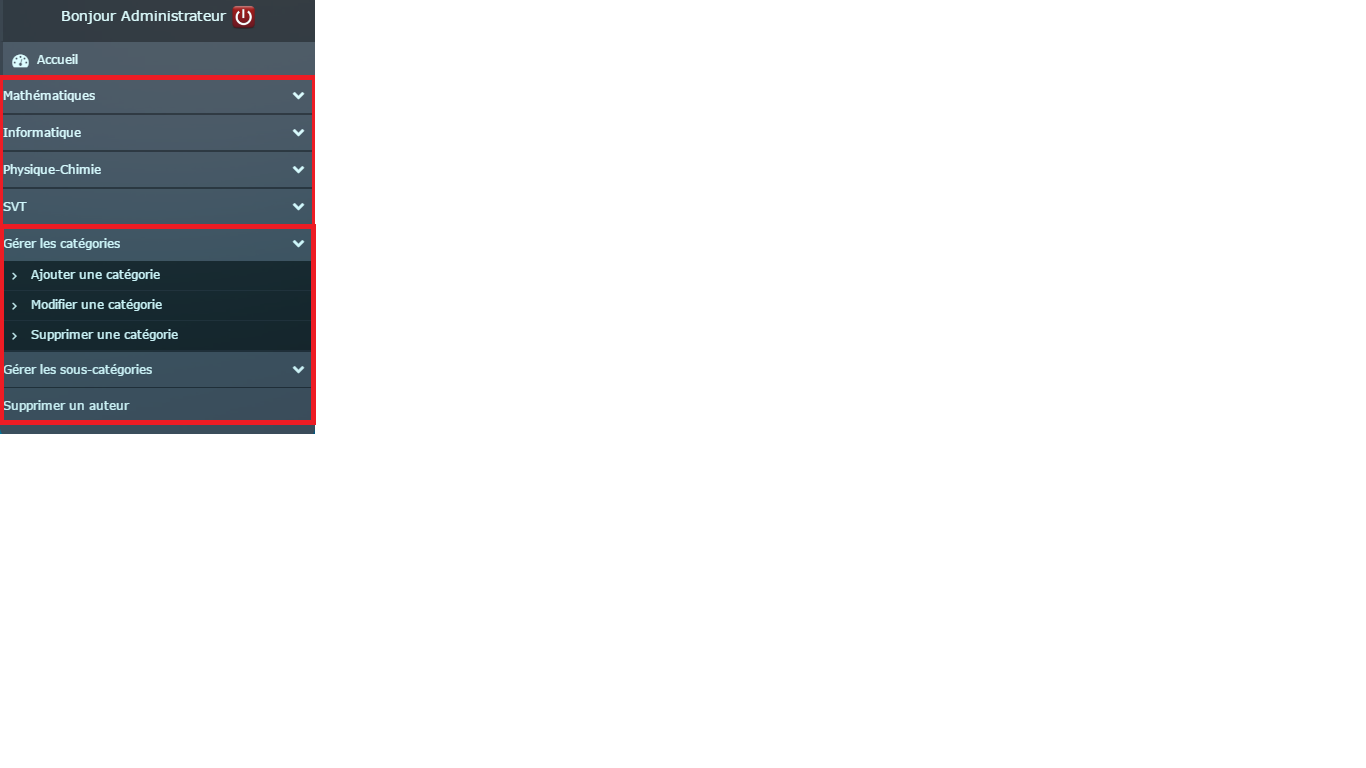
\includegraphics[width=8cm]{images/menu2.png}\\
\end{center}

Dans le premier encadré rouge, on voit l'arborescence générée automatiquement en fonction de la base de données. Dans le deuxième, on voit le menu de gestion pour l'administrateur.\\

Lors de l'administration, l'administrateur peut ajouter un nouveau élément (catégorie ou sous-catégorie), modifier le nom de cet élément ou supprimer cet élément s'il ne possède aucun fils.\\

A chaque fois qu'on envoie un formulaire, on modifie la base de données MENU grâce à des requêtes.\\

\newpage
\begin{center}
\textsc{Ajouter une catégorie}\\
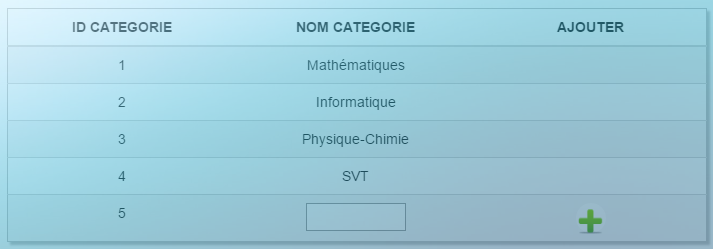
\includegraphics[width=16cm]{images/ajoutcat.png}\\
\end{center}

\begin{center}
\textsc{Modifier une sous-catégorie}\\
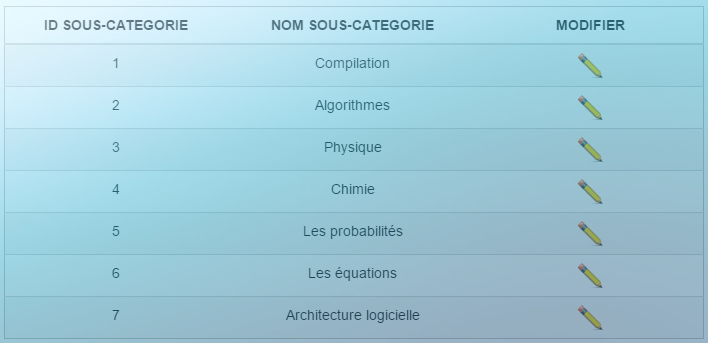
\includegraphics[width=16cm]{images/modifcateg.png}\\
\end{center}

\newpage
\begin{center}
\textsc{Valider la modification}\\
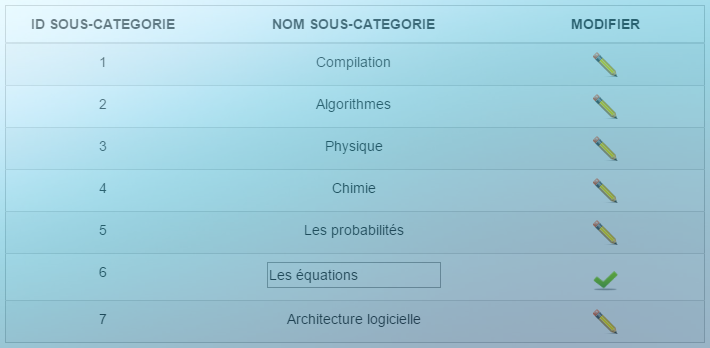
\includegraphics[width=16cm]{images/modifcateg2.png}\\
\end{center}

\begin{center}
\textsc{Supprimer une catégorie}\\
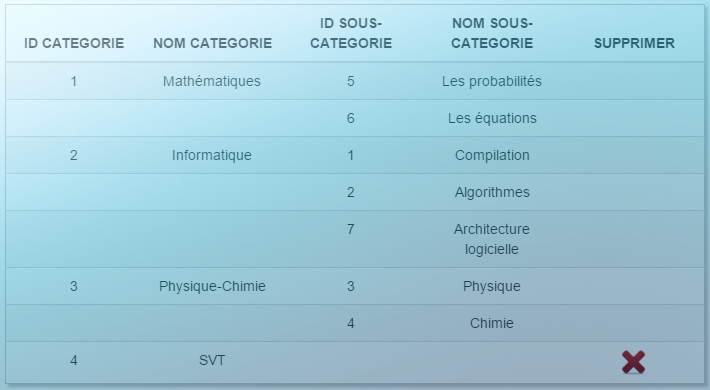
\includegraphics[width=16cm]{images/suppcat.png}\\
\end{center}

\subsubsection{Gérer les rédacteurs}
L'administrateur peut aussi supprimer les rédacteurs.

\begin{center}
\textsc{Supprimer un auteur}\\
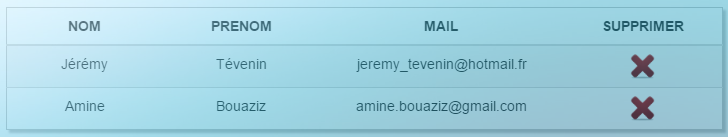
\includegraphics[width=16cm]{images/suppaut.png}\\
\end{center}

\newpage
\subsection{Par les rédacteurs}
\subsubsection{Créer un article}
Pour créer un article, le rédacteur doit choisir la sous-catégorie et un nom d'article. On ne peut pas créer un article avec un nom qui est déjà utilisé.

\begin{center}
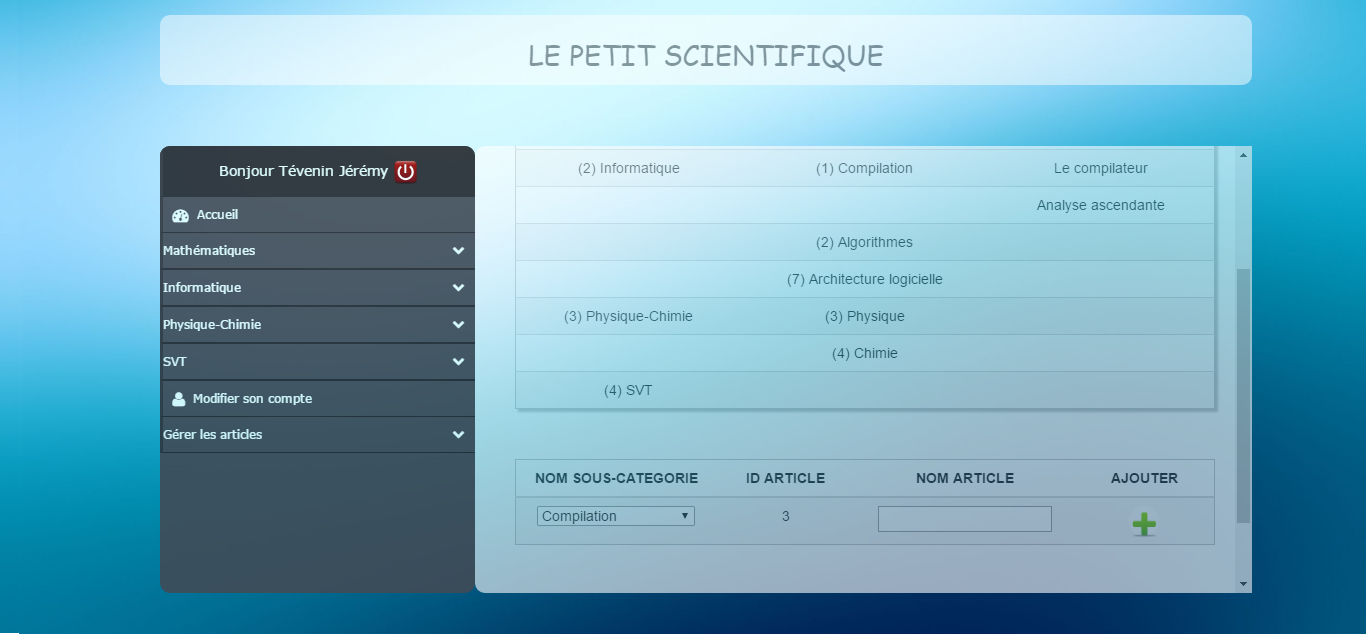
\includegraphics[width=16cm]{images/ajoutart.png}\\
\end{center}

\begin{center}
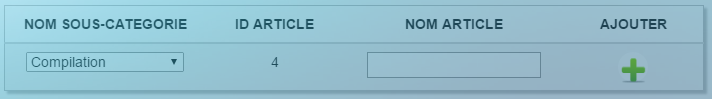
\includegraphics[width=16cm]{images/ajoutart2.png}\\
\end{center}

Pour rédiger un article, nous avons intégré l'éditeur CKeditor qui permet au rédacteur d'écrire ses articles.

\begin{center}
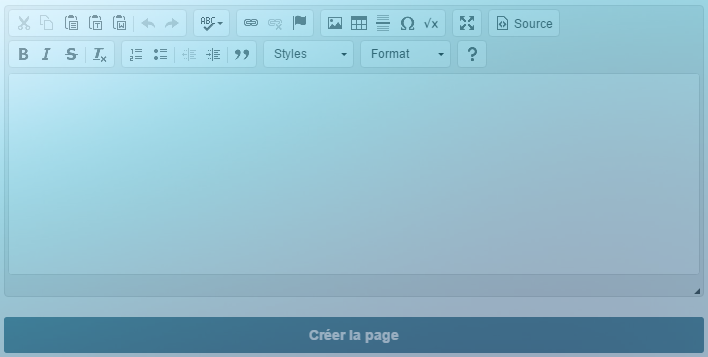
\includegraphics[width=16cm]{images/ajoutart3.png}\\
\end{center}

Lorsque le rédacteur a validé le contenu de son article, un répertoire au nom de l'article est créé dans le dossier articles. Un fichier php est créé et contient une fonction qui sera appelé pour afficher l'article.

\subsubsection{Modifier un article}
Un rédacteur ne peut modifier que le contenu de ses articles.\\

\begin{center}
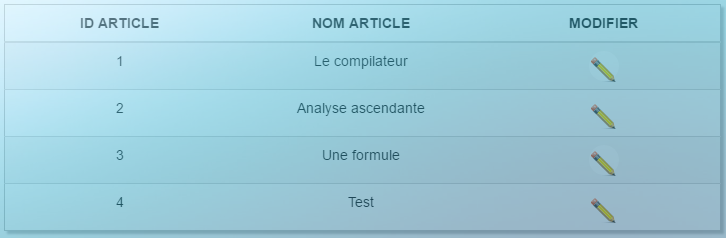
\includegraphics[width=16cm]{images/modifart.png}\\
\end{center}

\begin{center}
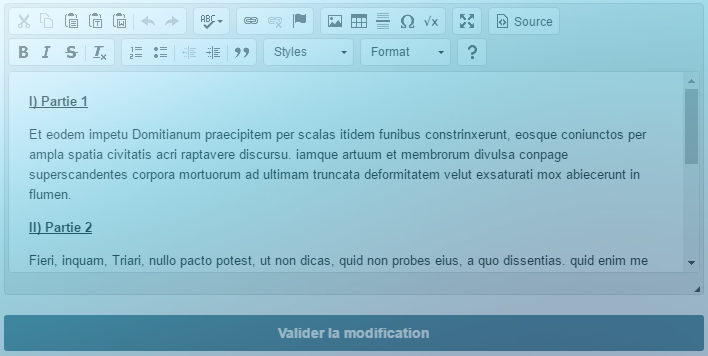
\includegraphics[width=16cm]{images/modifart2.png}\\
\end{center}


\subsubsection{Supprimer un article}
Un rédacteur ne peut supprimer que le contenu de ses articles.\\
\begin{center}
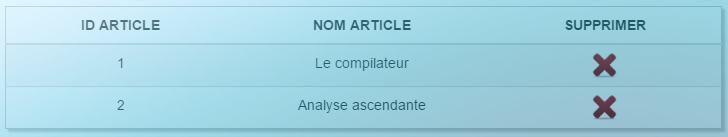
\includegraphics[width=16cm]{images/suppart.png}\\
\end{center}

Lorsque le rédacteur supprime un article, le répertoire contenant l'article est supprimé du dossier articles.

\subsubsection{Modifier son mot de passe}
Un rédacteur ne peut modifier son mot de passe.\\
\begin{center}

\includegraphics[width=16cm]{images/modifauteur.png}\\
\end{center}


\newpage
\section{Le style du site (CSS)}
Le CSS a été réalisé grâce au framework Bootstrap 3 qui nous a permis de réaliser un site plus ergonomique et harmonieux.
\subsection{Le site}
Nous avons majoritairement utilisé des \% afin que tous les éléments soit bien dimensionnés par rapport à la taille de l'écran.
\subsection{Le menu}
Nous avons réalisé ce menu grâce aux balises li et ul d'HTML. Voici un exemple de l’affichage du menu, bien sûr, de nombreuses boucles sont là pour automatiser l'affichage du menu. Cette fonction est entre une balise ouvrante <div> et une balise fermante </div>. 
Voici l'arborescence du menu déroulant. Une classe CSS lui a été défini afin de le rendre plus agréble et élégant.

<ul id="menu-content" class="menu-content collapse out">\\
   <li data-toggle="collapse" data-target="\#categ".cpt."" class="collapsed">\\
      Requête permettant d'obtenir le nom des catégories\\
     <ul class="sub-menu collapse" id="categ".cpt."">\\
           <li data-toggle="collapse" data-target="\#souscateg".cpt1."" class="collapsed">\\
                Requête permettant d'obtenir le nom des sous catégories\\
                 <ul class="sub-sub-menu collapse" id="souscateg".cpt1."">\\
                    <li data-toggle="collapse" data-target="\#article".cpt2."" class="collapsed ">\\
                        Requête récupérant les articles\\
                    </li>\\
               </ul>\\
          </li>\\
        </ul>\\
    </li>\\
</ul>\\

Nous avons utilisé la fonction "hover" de CSS. Cette fonction permet au menu quand il n'est pas activé par le passage de la souris de rester caché. Ce qui permet de faire un menu dynamique au passage de la souris. Nous avons aussi mis une couleur différente lorsque l'utilisateur navigue dans le menu pour qu'il voit dans quelle partie il se trouve.
Pour pouvoir afficher ce menu des requêtes sont effectuées.

\newpage
\section{Conclusion}
Ce projet nous a permis de mettre à profit nos compétences et connaissances en Web grâce notamment aux differents TPs vus ce semestre. Nous avons donc pu grâce à ça, developper notre site en modèle MVC. Bien sûre, notre projet peut recevoir des améliorations comme par exemple l'implémentation de notre propre éditeur de texte. Toutes nos pages ainsi que le CSS sont validées par le W3C.

\end{document}
